\documentclass{"../../res/univ-projet"}
\usepackage[utf8]{inputenc}
\usepackage[T1]{fontenc}
\usepackage[francais]{babel}
\usepackage{colortbl}
\usepackage{algorithm}
\usepackage{algorithmic}


\logo{../../res/logo_univ.png}
\title{Architecture Logicielle}
\author{Damien \bsc{Picard}, Tayewo John Yves \bsc{Adegoloye}}
\projet{M1SSI}
\projdesc{Projet de génération d'OTP}
\filiere{M1SSI}
\version{2.0}
\relecteur{Adrien \bsc{Smondack}}
\signataire{\bsc{Bardet} Magali}
\date{Février 2014}

\histentry{2.0}{18/02/2014}{Version post état de l'art}
\histentry{1.2}{16/01/2014}{Version pour la revue de lancement}
\histentry{1.1}{15/12/2013}{Ajout des modifications demandées par le client}
\histentry{1.0}{01/12/2013}{Version relue et corrigée}
\histentry{0.1}{21/11/2013}{Premier jet}


\begin{document}
\maketitle
%-------------------------------------------------------------------------------
\section{Objet}
Ce document a pour but de préciser les détails techniques du logiciel final.

\section{Documents de référence}
\subsection{Documents de spécifications}
\begin{tabular}{p{1,5cm}>{\raggedright\arraybackslash}p{13cm}}
    {[ANS10]} & {ANSSI. Référentiel général de sécurité. \href{http://www.ssi.gouv.fr/fr/reglementation-ssi/referentiel-general-de-securite}{http://www.ssi.gouv.fr/fr/reglementation-ssi/referentiel-general-de-securite}, 2010.}
    \tabularnewline
    \\
    {[MvOV97]} & {Alfred J. Menezes, Paul C. van Oorschot, and Scott A. Vanstone. Handbook of applied cryptography. CRC Press Series on Discrete Mathematics and its Applications. CRC Press, Boca Raton, FL, 1997. With a foreword by Ronald L.Rivest.}
    \tabularnewline
    \\
    {[RFC98]} & {A One-Time Password System. \href{http://tools.ietf.org/html/rfc2289}{http://tools.ietf.org/html/rfc2289}, 1998.}
    \tabularnewline
    \\
    {[RFC05]} & {HOTP:An HMAC-Based One-Time Password Algorithm \href{http://tools.ietf.org/html/rfc4226}{http://tools.ietf.org/html/rfc4226}, 2005.}
    \tabularnewline
    \\
    {[RFC06]} & {Generic Message Exchange Authentication for the Securer Shell Protocol (SSH).\href{http://tools.ietf.org/html/rfc4256}{http://tools.ietf.org/html/rfc4256}, 2006.}
    \tabularnewline
    \\
    {[RFC07]} & {The EAP Protected One-Time Password Protocol (EAP-POTP). \href{http://tools.ietf.org/html/rfc4793}{http://tools.ietf.org/html/rfc4793}, 2007.}
    \tabularnewline
    \\
    {[RFC11]} & {HOTP: Time-Based One-Time Password Algorithm \href{http://tools.ietf.org/html/rfc6238}{http://tools.ietf.org/html/rfc6238}, 2011.}
    \tabularnewline
    \\
    {[goo]} & {Google Authenticator \href{https://code.google.com/p/google-authenticator/}{https://code.google.com/p/google-authenticator/}.}
    \tabularnewline
    \\
\end{tabular}

%-------------------------------------------------------------------------------
\section{Configuration requise}

\subsection{Périphériques et matériel spécifiques}
\begin{tabular}{|p{0.2\textwidth}|p{0.4\textwidth}|p{0.4\textwidth}|}
    \hline
    \rowcolor{gray}
    \textcolor{white}{\bfseries Identifiant} & 
    \textcolor{white}{\bfseries Description} &
    \textcolor{white}{\bfseries Justification} \\
    \hline
    PR-M\_001 &
    Calculateur \verb?700MHz? pour le token &
    Étant donné que le calcul de l'OTP ne prend que très peu de ressources
    et que les plateformes sont diverses le critère des \verb?700MHz? de puissances
    de calcul paraît un bon facteur commun.\\
    \hline
    PR-M\_002 &
    Communication stable entre le client et le serveur &
    La communication stable entre le client et le serveur permet d'assurer que si
    il y a un problème lors de l'authentification ce n'est pas du à une perte de
    connexion lors de la requête d'authentification.\\
    \hline
\end{tabular}

\subsection{Système d'exploitation}
\begin{tabular}{|p{0.2\textwidth}|p{0.4\textwidth}|p{0.4\textwidth}|}
    \hline
    \rowcolor{gray}
    \textcolor{white}{\bfseries Identifiant} & 
    \textcolor{white}{\bfseries Description} &
    \textcolor{white}{\bfseries Justification} \\
    \hline
    OS\_001& 
    GNU/Linux kernel 3.x / glibc >= 2.15, présence de /dev/random et /dev/urandom 
    pour un module PAM&
    Le but du projet est de développer un module PAM pour pouvoir s'authentifier
    à l'aide de mot de passe jetable. PAM est une technologie qui n'est disponible
    que sur certains systèmes de type UNIX.\\
    \hline
    OS\_002&
    Android 2.3.x comptabile 4.x pour un token&
    Ceci est dans le cas de l'implantation sur une plateforme type
    smartphone. Une fois de plus ce choix se justifie par
    l'aspect libre du système et le matériel disponible.\\
    \hline
\end{tabular}

\subsection{Pré-requis logiciels}
\begin{tabular}{|p{0.2\textwidth}|p{0.4\textwidth}|p{0.4\textwidth}|}
    \hline
    \rowcolor{gray}
    \textcolor{white}{\bfseries Identifiant} & 
    \textcolor{white}{\bfseries Description} &
    \textcolor{white}{\bfseries Justification} \\
    \hline
    PR-L\_001 &
    Support de l'API POSIX pour le token, le client et le serveur &
    Ceci va de pair avec le choix de GNU/Linux comme système d'exploitation,
    c'est une technologie libre et performante.\\
    \hline
    PR-L\_002 &
    Un moyen de stocker les informations relatives aux utilisateurs dans le serveur&
    Cela sera nécessaire pour gérer plusieurs utilisateurs ainsi que plusieurs protocoles
    OTP pour le serveur.\\
    \hline
    PR-L\_003 &
    PAM > 1.0 &
    Afin d'assurer la compatibilité entre PAM et notre module nous utiliserons
    une version de PAM supérieure à 1.0.\\
    \hline
\end{tabular}


%-------------------------------------------------------------------------------
\part*{Architectures statiques}
\section{Structure générale du système}
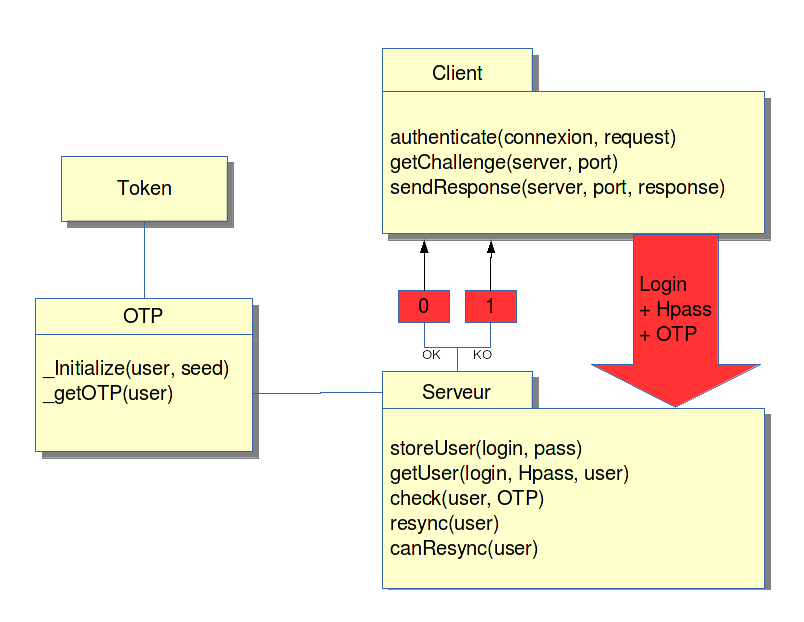
\includegraphics[width=\textwidth]{../graphics/architecture.png}

\subsection{Token}
    \subsubsection{Rôle}
        Afficher les mots de passe jetables pour un utilisateur donné.

    \subsubsection{Propriétés et attributs de caractérisation}
    \begin{description}
        \item[Secret] Le secret de l'utilisateur qui permet de générer les
            mots de passe jetables.
        \item[User] La structure qui contient les données de l'utilisateur.
            Stockée dans la mémoire à long terme du support.
    \end{description}

    \subsubsection{Dépendances}
        \begin{itemize}
            \item Générateurs d'OTP.
            \item Toolkit d'interaction avec l'utilisateur.
        \end{itemize}

    \subsubsection{Langages de programmation}
        Les langages utilisés pour créer des tokens seront: le C pour GNU/Linux,
    et Java pour Android. Dans le cas de JavaCard (optionnel) il n'y a pas besoin
    de tokens puisque c'est la carte qui fournit ce service.

    \subsubsection{Procédés de développement}
    \begin{enumerate}
        \item Développer des modules réalisant chaque algorithme de génération
            d'OTP.
	\item Permettre une gestion de plusieurs services. C'est à dire
	  faire en sorte que le token puisse stocker plusieurs secret
	  pour différents services.
        \item Permettre une interaction avec l'utilisateur.
    \end{enumerate}

    \subsubsection{Taille et complexité}
            Taille et complexité dépendantes de l'algorithme de génération
        de mots de passe jetables.

%------------------------------------------------------------------------------
\subsection{Générateur d'OTP}
    Chaque algorithme étudié et implémenté (HOTP, TOTP) offrira les
    mêmes services, seul le fonctionnement interne du module diffèrera.
    les algorithmes seront détaillés dans les dossiers associés aux recherches sur 
    chaque algorithme.
    
        Chaque protocole choisi fera l'objet de l'implémentation d'une bibliothèque
    logicielle permettant de s'intégrer dans un serveur et un token.
    \subsubsection{Rôle}
        Générer des mots de passe jetables à partir d'un secret permettant
    de s'authentifier.

    \subsubsection{Services offerts}
      Ce module n'offre qu'un unique service, générer un OTP à partir d'un secret et
    d'un état du générateur. Pour HOTP cet état est représenté par un compteur.

    \subsubsection{Langages de programmation}
    Pour créer les tokens GNU/Linux, nous utiliserons le langage C.
    Pour créer les tokens Android nous utiliserons le langage Java.
    Dans le cas de JavaCard (optionnel) c'est aussi le langage Java qui sera
    utilisé.

    \subsubsection{Procédé de développement}
    \begin{enumerate}
        \item Développer des modules réalisant chaque algorithme de génération
            d'OTP.
    \end{enumerate}

    \subsubsection{Taille et complexité}
            Taille et complexité dépendantes de l'algorithme de génération
        de mots de passe jetables, mais suffisamment faibles pour tenir sur
        de petites capacités mémoire et permettre un calcul 
        en t < 1s sur \verb?700MHz?.

\subsection{Vérificateur d'OTP}
  \subsubsection{Rôle}
    Vérifier qu'un OTP permet de s'authentifier sur un service.
    
  \subsubsection{Services offerts}
    Ce module n'offre qu'un service, vérifier un OTP avec un secret
    et un état. Ce module va s'appuyer sur les services offerts par
    un générateur d'OTP et vérifier que les données correspondent.
    
  \subsubsection{Langage de programmation}
    Ce module n'étant utile qu'au module PAM il ne sera implémenté qu'en C.
    
  \subsubsection{Procédé de développement}
  \begin{enumerate}
   \item Développer les générateurs d'OTP.
   \item Développer une gestion des utilisateurs.
   \item Développer la fonction de vérification.
   \item Développer la fonction de resynchronisation.
  \end{enumerate}
  
  \subsubsection{Taille et complexité}
  La encore la taille et la complexité sont dépendantes de l'algorithme 
  choisi. Mais on peut estimer la taille et la complexité des Vérificateurs
  comme étant identique à celle des générateurs. De plus la présence d'une fonction
  de resynchronisation représente un  vecteur d'attaque (possibilité de synchroniser
  sur une valeur non désirée), il faut donc ajouter un certain nombre de vérifications.
  
  
\subsection{Le module PAM}
\subsubsection{Rôle}
  Ce module permettra de s'authentifier sur un système en utilisant un mot de passe
  jetable. L'avantage de développer un module PAM est que de nombreux services existants
  peuvent s'interfacer avec PAM: services web avec php, ssh, ... De plus il est assez
  aisé de développer ultérieurement une application qui gère son authentification à l'aide de PAM.
  Enfin il sera possible d'intégrer le module au sein d'une authentification existante ce qui permettra
  de créer une authentification à plusieurs facteurs.
  
  
\subsubsection{Services offert}
  Ce module devra gérer la vérification de la validité d'un OTP pour un utilisateur donné ainsi que la
  mise à jour des données relatives à cet utilisateur.
  
\subsubsection{Gestion des utilisateurs}
  Afin de gérer les utilisateurs le module PAM créera un fichier sur le système.
  Ce fichier contiendra une ligne par utilisateurs avec:
  \begin{itemize}
   \item Le login de l'utilisateur.
   \item Le secret de l'utilisateur.
  \end{itemize}
  
  Dans notre cas le secret est déterminé par le système distant. Il doit
  cependant être possible de réinitialiser ce secret. 
  
\subsubsection{Langage de programmation}
  C'est un module PAM donc le langage est imposé, nous utiliserons le C.
  
\subsubsection{Procédé de développement}
  Pour la partie authentification, le module PAM est complètement
  dépendant de la vérification des OTP qui elle est dépendante de la 
  génération d'OTP et de la gestion d'utilisateurs.

  Pour la partie mise à jour de crédentials il faut générer une clé aléatoire
  à l'aide de /dev/random puis la dériver.
  
\subsubsection{Taille et complexité}
  Cette partie correspond à la liaison des étapes précédentes. Sa taille et
  sa complexité sont donc assez faibles.
  
\subsection{Justification des choix techniques}
\subsubsection{Le langage C}
Le langage C a été choisi pour 2 raisons:
\begin{enumerate}
    \item Car il est supposé connu de tout les membres de l'équipe, au vu
        de l'enseignement reçu.
    \item Les modules PAM ne peuvent être programmés qu'en C.
\end{enumerate}

\subsubsection{Le langage Java}
    Le langage Java sera utilisé sur les plateformes Android
    et Javacard, car bien qu'il soit possible de programmer en C
    sur Android, ce n'est pas recommandé par \verb?Google?
    \footnote{\href{https://developer.android.com/tools/sdk/ndk/index.html}{Android NDK}}.
        
\part*{Architecture dynamique}

\section{Demande de secret}
\subsection{Principe}
Le secret doit être partagé entre le système hôte et le token. Pour déterminer
le secret il faut faire une demande au système hôte. Ce dernier possède une clé
maîtresse qu'il dérivera pour donner une nouvelle clé à l'utilisateur. L'utilisateur
devra entrer le secret lui même sur le token.


\section{Authentification}
\subsection{Principe}
L'utilisateur tente de s'authentifier sur un service, ce service appelle PAM. 
PAM va charger les modules correspondants à la configuration pour le service.
Et vérifier l'OTP passé au service. Dans le cas où le token est désynchronisé
avec le module PAM une opération de resynchronisation a lieu.

\subsection{Resynchronisation}
\subsubsection{Principe}
Le serveur se resynchronise sur le token pour être d'accord sur la suite des
mots de passe jetables générés.

\subsubsection{Fonctionnement}
\begin{enumerate}
    \item L'utilisateur essaie de s'authentifier.
    \item L'OTP fourni par l'utilisateur n'est pas valide.
    \item Deux cas possibles:
    \begin{itemize}
    	\item L'OTP correspond à un OTP dans une fenêtre de $n$ OTP.
    		auquel cas les données de l'utilisateur dans le fichier
    		/var/otpwd sont resynchronisées.
    	\item L'OTP ne correspond pas un de ces OTP.
    \end{itemize}
\end{enumerate}
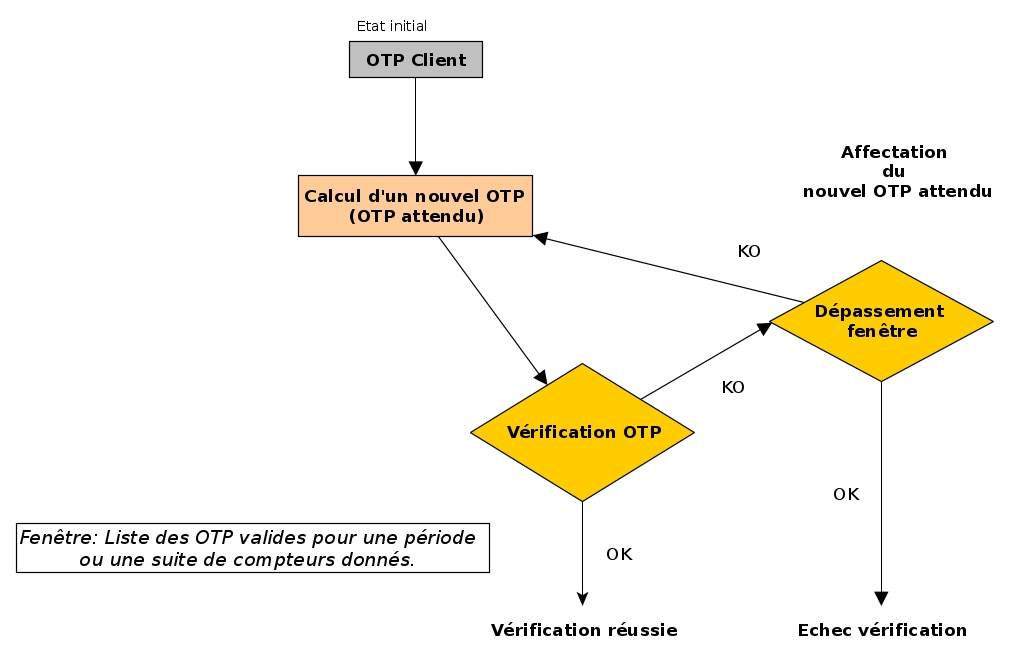
\includegraphics[width=\textwidth]{../graphics/resynchronisation.jpg}
\end{document}

\subsection{Description graphique}
% TODO mettre le graph
